\section{Nonsmooth Optimization}

\subsection{Convex Conjugacy}

	\begin{definition}[Proper Functions]
		Given a function $f: \mathbb{R}^d \to (-\infty, +\infty]$, it is called \textbf{proper} if it is finite somewhere. The \textbf{effective domain} is 
		\begin{equation}
			\dom(f) \coloneqq \{ x \in \mathbb{R}^d \colon f(x) < +\infty \}
		\end{equation}
	\end{definition}

	\begin{definition}[Convex, Fenchel Conjugate]
		Given a proper function $f: \mathbb{R}^d \to (-\infty, +\infty]$, its \textbf{convex conjugate}, or \textbf{Fenchel conjugate}, is defined to be 
		\begin{equation}
			f: \{y \colon f^\ast (y) < +\infty\} \to \mathbb{R}, \quad f^\ast (y) = \sup_{x \in \mathbb{R}^d} \{ \langle y, x \rangle - f(x) \}
		\end{equation}
		satisfying 
		\begin{enumerate}
			\item \textit{Convexity}. For all $x, y \in \mathbb{R}^d$, $f(tx + (1 - t)y) \leq t f(x) + (1 - t) f(y)$. 
			\item \textit{Lower Semicontinuous}. 
		\end{enumerate}
	\end{definition}
	\begin{proof}
	  It is a pointwise supremum of continuous affine functions of $y$. 
	\end{proof}

	This generalizes the classical Legendre transform. 

	\begin{theorem}[Fenchel-Young Inequality]
		Let $f$ be a proper function and $f^\ast$ its convex conjugate. For every $x \in \dom(f)$ and $y \in \mathbb{R}^d$\footnote{We don't need to restrict to $y \in \dom(f^\ast)$.}, 
		\begin{equation}
		  f(x) + f^\ast (y) \geq \langle y, x \rangle
		\end{equation}
	\end{theorem}
	\begin{proof}
	  
	\end{proof}

	\begin{definition}[Subgradients, Subdifferentials]
		Given proper function $f$, a vector $y \in \mathbb{R}^d$ is a \textbf{subgradient} of $f$ at $x \in \dom(f)$ if 
		\begin{equation}
			f(z) \geq f(x) + \langle y, z - x \rangle \quad \forall z \in \mathbb{R}^d
		\end{equation}
		The set of all subgradients at $x$ is the \textbf{subdifferential} 
		\begin{equation}
			\partial f(x) \coloneqq \{ y \in \mathbb{R}^d \colon f(z) \geq f(x) + \langle y, z - x \rangle \; \forall z \}
		\end{equation}
	\end{definition}

  It is well known that the mean square error of a linear map is convex. However, when we impose---say the L1 penalty---the loss function is now not differentiable at $0$. The subgradient also acts as a linear approximation of $f$, but now at nondifferentiable points of convex functions, we have a set of linear approximations. It is clear that the subgradient at a differentiable point is uniquely the gradient ($\partial f(\mathbf{x}) = \{ \nabla f(\mathbf{x})$), but for places like the absolute value, we can have infinite linear approximations. 

	\begin{example}[Subgradients of Absolute Value Function]
    The subdifferential of the absolute value function $f(x) = |x|$ at any given $x$ is 
    \begin{equation}
      \partial f(x) = \begin{cases} 1 & \text{ if } x > 0 \\ [-1, 1] & \text{ if } x = 0 \\ -1 & \text{ if } x < 0 \end{cases}
    \end{equation}

		\begin{figure}[H]
			\centering 
			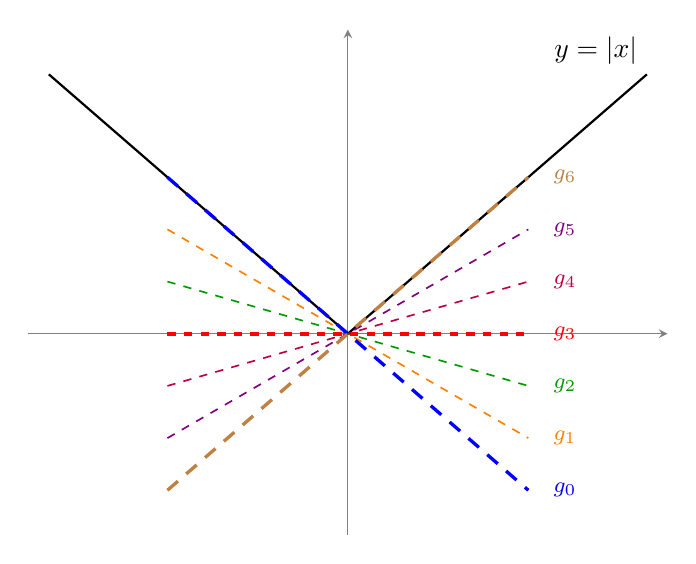
\begin{tikzpicture}
				\begin{axis}[
					width=0.8\textwidth, height=8cm,
					axis lines=middle,
					xmin=-0.62, xmax=0.62, ymin=-0.45, ymax=0.68,
					xtick=\empty, ytick=\empty,
					clip=false,
					axis line style={gray}
				]
					% y = |x|
					\addplot[domain=-0.58:0.58, samples=201, thick, black] {abs(x)};
					\node[anchor=south east] at (axis cs:0.58,0.58) {$y = |x|$};

					% the subgradients g = mx for m ranging over [-1, 1]; the extreme
					% slopes m = \pm 1 lie along the two arms of |x| itself.
					\addplot[domain=-0.35:0.35, dashed, semithick, orange]        {-2*x/3};
					\addplot[domain=-0.35:0.35, dashed, semithick, green!60!black] {-x/3};
					\addplot[domain=-0.35:0.35, dashed, ultra thick, red]          {0};
					\addplot[domain=-0.35:0.35, dashed, semithick, purple]         {x/3};
					\addplot[domain=-0.35:0.35, dashed, semithick, violet]         {2*x/3};
					\addplot[domain=-0.35:0.35, dash pattern=on 5pt off 4pt, very thick, blue]  {-x};
					\addplot[domain=-0.35:0.35, dash pattern=on 5pt off 4pt, very thick, brown] {x};

					\node[anchor=west, font=\footnotesize, blue]           at (axis cs:0.38,-0.35)   {$g_0$};
					\node[anchor=west, font=\footnotesize, orange]         at (axis cs:0.38,-0.2333) {$g_1$};
					\node[anchor=west, font=\footnotesize, green!60!black] at (axis cs:0.38,-0.1167) {$g_2$};
					\node[anchor=west, font=\footnotesize, red]            at (axis cs:0.38,0)       {$g_3$};
					\node[anchor=west, font=\footnotesize, purple]         at (axis cs:0.38,0.1167)  {$g_4$};
					\node[anchor=west, font=\footnotesize, violet]         at (axis cs:0.38,0.2333)  {$g_5$};
					\node[anchor=west, font=\footnotesize, brown]          at (axis cs:0.38,0.35)    {$g_6$};
				\end{axis}
			\end{tikzpicture}
			\caption{} 
			\label{fig:subgradient_abs}
		\end{figure}
  \end{example}

  Given the subdifferential, thus the optimality condition for any convex $\mathbf{f}$ (differentiable or not) is
  \begin{equation}
    f(\mathbf{x}^\ast) = \min_{\mathbf{x}} f(\mathbf{x}) \iff \mathbf{0} \in \partial f(\mathbf{x}^\ast)
  \end{equation}
  known as the subgradient optimality condition. 

	\begin{theorem}[Equality in Fenchel-Young]
	  For any proper $f$ and $x \in \dom(f)$, 
		\begin{equation}
		  f(x) + f^\ast (y) = \langle y, x \rangle \iff y \in \partial f(x)
		\end{equation}
	\end{theorem}
	\begin{proof}
	  
	\end{proof}

	\begin{definition}[Biconjugate]
		Given proper $f$ and its convex conjugate $f^\ast$, the \textbf{biconjugate} of $f$ is the conjugate of $f^\ast$. 
		\begin{equation}
			f^{\ast\ast} (x) = \sup_{y \in \mathbb{R}^d} \{ \langle y, x \rangle - f^\ast (y) \}
		\end{equation}
	\end{definition}

	\begin{corollary}[Affine Lower Bound Reconstruction]
		Given proper $f$, we have 
		\begin{equation}
			f^{\ast\ast} \leq f
		\end{equation}
		That is, $f^{\ast\ast}$ reconstructs $f$ from its affine lower bounds. 
	\end{corollary}

	\begin{theorem}[Fenchel-Moreau]
	  If $f$ is proper, then the following are equivalent. 
		\begin{enumerate}
			\item $f = f^{\ast\ast}$. 
			\item $f$ is convex and lower-semicontinuous. 
		\end{enumerate}
	\end{theorem}
	\begin{proof}
	  
	\end{proof}

	Therefore, a proper lower semicontinuous convex function can be recovered entirely from its conjugate. 

	\begin{theorem}[Reciprocity of Subgradients]
	  If $f$ is proper, lower-semicontinuous, and convex, then the following are equivalent. 
		\begin{enumerate}
		  \item $y \in \partial f(x)$. 
			\item $x \in \partial f^\ast (y)$. 
			\item $f(x) + f^\ast (y) = \langle y, z \rangle$. 
		\end{enumerate}
	\end{theorem}
	\begin{proof}
	  
	\end{proof}

\subsection{Subgradient Descent}

	Since $\partial f(x)$ is a \textit{set}, the first-order oracle of the smooth case no longer makes sense: there is nothing for $\mathcal{O}_f(x)$ to return at a point where $f$ is kinked. We must fix a choice.

	\begin{definition}[Weak Subgradient Oracle]
		\label{def:weak_subgradient_oracle}
		Let $\mathcal{F}$ be the class of proper convex functions $f : S \subset \mathbb{R}^d \to \mathbb{R}$. A \textbf{subgradient selection} for $f$ is any map
		\begin{equation}
			g_f : S \to \mathbb{R}^d, \quad g_f(x) \in \partial f(x) \quad \forall x \in S
		\end{equation}
		and the \textbf{weak subgradient oracle} associated with it is
		\begin{equation}
			\mathcal{O}_f : S \to \mathbb{R} \times \mathbb{R}^d, \quad \mathcal{O}_f (x) = \big( f(x), g_f(x) \big)
		\end{equation}
	\end{definition}

	Unlike the first-order oracle, $\mathcal{O}_f$ is \textit{not} determined by $f$ alone, since a proper convex $f$ admits many selections---in Figure \ref{fig:subgradient_abs}, any of the $g_i$ is a legal answer at $x = 0$. The convention is that an algorithm must work for \textit{every} admissible selection, i.e. the oracle is free to return the worst element of $\partial f(x_t)$ at each query. This is what makes the model a fair one for proving lower bounds. At any $x$ where $f$ is differentiable, $\partial f(x) = \{\nabla f(x)\}$, the selection is forced, and we recover the first-order oracle exactly.

	\begin{definition}[Subgradient Descent]
		\label{def:subgradient_descent}
		Let $\mathcal{F}$ be the class of proper convex functions $f: S \subset \mathbb{R}^d \to \mathbb{R}$ that are $G$-Lipschitz, i.e. $\|g\| \leq G$ for every $x \in S$ and every $g \in \partial f(x)$. Fix an initial point $x_0 \in S$, a sequence of positive step sizes $(\eta_t)$, and a \hyperref[def:weak_subgradient_oracle]{weak subgradient oracle}
		\begin{equation}
			\mathcal{O}_f : S \to \mathbb{R} \times \mathbb{R}^d, \quad \mathcal{O}_f (x) = \big( f(x), g_f(x) \big), \quad g_f(x) \in \partial f(x)
		\end{equation}
		Then \textbf{subgradient descent} is a deterministic algorithm defined by $\mathcal{O}_f$ and update maps $\Phi_t : (S \times (\mathbb{R} \times \mathbb{R}^d))^{t+1} \to S$
		\begin{align}
			x_{t+1} = \Phi_t \big( x_0, (f(x_0), g_0), \ldots, x_t, (f(x_t), g_t) \big)
				& \coloneqq x_t - \eta_t g_t \\
				& = \argmin_w \bigg\{ \underbrace{\langle g_t, w - x_t \rangle}_{\text{affine minorant}} + \underbrace{\frac{1}{2\eta_t} \|w - x_t\|^2}_{\text{anchor}} \bigg\}
		\end{align}
		where $g_t \coloneqq g_f(x_t) \in \partial f(x_t)$. After $k$ iterations, the output rule $\Psi_k$ returns either the \textbf{best iterate}
		\begin{equation}
			w_{\mathcal{A}_k} (f) = x_{t^\ast}, \quad t^\ast = \argmin_{0 \leq t \leq k} f(x_t)
		\end{equation}
		or the step-size weighted \textbf{ergodic average}
		\begin{equation}
			w_{\mathcal{A}_k} (f) = \bar{x}_k \coloneqq \frac{\sum_{t=0}^k \eta_t x_t}{\sum_{t=0}^k \eta_t}
		\end{equation}
	\end{definition}

	The update is the verbatim analogue of \hyperref[def:gradient_descent]{gradient descent}: minimize an affine model of $f$ plus a quadratic anchor. The only change is that the model is now a genuine \textit{global lower bound} on $f$, by the very definition of the subgradient, rather than a local Taylor approximation. Two other parts of the definition, however, really do differ from the smooth case, and both are forced on us rather than chosen.

	\textit{First, the output rule cannot be $w_{\mathcal{A}_k}(f) = x_k$.} Despite its name, subgradient descent is \textbf{not a descent method}. Where $f$ is nondifferentiable, $-g_t$ need not be a descent direction at all, so $f(x_{t+1}) > f(x_t)$ can happen for \textit{every} positive step size.

	\begin{example}
		Let $f(x_1, x_2) = |x_1| + 2|x_2|$ and take $x_t = (1, 0)$, so that $f(x_t) = 1$. Here $\partial f(x_t) = \{1\} \times [-2, 2]$, so $g_t = (1, 2)$ is a legal oracle response. Then $x_{t+1} = (1 - \eta, -2\eta)$ and
		\begin{equation}
			f(x_{t+1}) = |1 - \eta| + 4\eta = 1 + 3\eta > 1 = f(x_t)
		\end{equation}
		for every $0 < \eta \leq 1$. The objective increases no matter how small the step.
	\end{example}

	So $(f(x_t))_t$ is not monotone, and the final iterate carries no guarantee on its own. Taking the running minimum or averaging is what restores one, and both achieve the rate below.\footnote{The last iterate \textit{does} converge under carefully chosen schedules, but this is a considerably harder result than the averaged case (Shamir and Zhang, 2013).}

	\textit{Second, the step sizes cannot be constant.} With $\eta_t = \eta$ fixed, the iterates only reach a neighborhood of the optimum: the error bound floors out at $\eta G^2 / 2$, and no amount of further iteration removes it. The standard requirement is that $(\eta_t)$ be diminishing but nonsummable,
	\begin{equation}
		\eta_t \to 0, \quad \sum_{t=0}^\infty \eta_t = \infty
	\end{equation}
	which drives the floor to $0$ while still letting the iterates travel an unbounded distance from $x_0$.

	\begin{theorem}[Convergence of Subgradient Descent]
		Let $f$ be convex and $G$-Lipschitz with minimizer $x^\ast$, and set $R = \|x_0 - x^\ast\|$. Running \hyperref[def:subgradient_descent]{subgradient descent} for a fixed horizon $k$ with the step size $\eta = \frac{R}{G \sqrt{k}}$ gives
		\begin{equation}
			\min_{0 \leq t \leq k} f(x_t) - f(x^\ast) \leq f(\bar{x}_k) - f(x^\ast) \leq \frac{GR}{\sqrt{k}}
		\end{equation}
	\end{theorem}
	\begin{proof}

	\end{proof}

	This $O(1/\sqrt{k})$ rate is far worse than the $O(1/k)$ that \hyperref[def:gradient_descent]{gradient descent} achieves on $L$-smooth convex functions, and it cannot be improved: it is the minimax rate over the class of $G$-Lipschitz convex functions in the black-box first-order model, so no cleverer choice of $\Phi_t$ and $\Psi_k$ does better. Note also that \hyperref[def:gradient_descent_momentum]{momentum} buys us nothing here. The gap is the price of nonsmoothness alone, which motivates the proximal methods of the next section: rather than probing the nonsmooth part of the objective with a subgradient, we handle it exactly.

\subsection{Proximal Methods}

  \begin{definition}[Proximal Operator]
    Given a lower semicontinuous convex function $f$ mapping from Hilbert space $X$ to $[-\infty, +\infty]$, its \textbf{proximal operator} associated with a point $u$ is defined 
    \begin{equation}
      \prox_{f, \tau} (u) = \argmin_{x} \bigg( f(x) + \frac{1}{2\tau} ||x - u||^2 \bigg)
    \end{equation}
    where $\tau > 0$ is a parameter that scales the quadratic term. This is basically the point that minimizes the sum of $f(x)$ and the square of the Euclidean distance between $x$ and $u$, scaled by $1/2\tau$. 
  \end{definition}

  Now given the loss function $L (\boldsymbol{\theta}) = L_{\mathrm{obj}} (\boldsymbol{\theta}) + L_{\mathrm{reg}} (\boldsymbol{\theta})$, we want to compute the proximal operator on the regularization loss and update that with the gradient of the smooth objective loss. 
  \begin{equation}
    \boldsymbol{\theta}^{(k+1)} = \prox_{L_{\mathrm{reg}}, \tau} \big[ \boldsymbol{\theta}^{(k)} - \tau \nabla L_{\mathrm{obj}} (\boldsymbol{\theta}^{(k)}) \big]
  \end{equation}
  Let's compute the proximal operator of the L1 loss $h(\boldsymbol{\theta}) = \lambda ||\boldsymbol{\theta}||_1$. We can parameterize this loss by the $\lambda$, so we will use the notation $\prox_{\lambda, \tau}$ rather than $\prox_{h, \tau}$. 
  \begin{align*}
    \prox_{\lambda, \tau} (\mathbf{u}) & = \argmin_{\boldsymbol{\theta}} \bigg( \lambda ||\boldsymbol{\theta}||_1 + \frac{1}{2\tau} ||\boldsymbol{\theta} - \mathbf{u}||_2^2 \bigg) \\
    & = \argmin_{\boldsymbol{\theta}} \bigg( \sum_{i=1}^n \lambda |\theta_i| + \frac{1}{2\tau} (\theta_i - u_i)^2 \bigg) 
  \end{align*}
  These are separable functions that can be decoupled and optimized component-wise. So, we really just want to find 
  \begin{equation}
    \theta_i^\ast = \argmin_{\theta_i} \bigg( \lambda |\theta_i| + \frac{1}{2\tau} (\theta_i - u_i)^2 \bigg)
  \end{equation}
  The sum of convex functions is convex, and so we should differentiate it and find where the gradient is $0$ to optimize it. 
  \begin{enumerate}
    \item When $\theta_i > 0$, then we minimize $\lambda \theta_i + \frac{1}{2\tau} (\theta_i - u_i)^2$, so taking the gradient and setting to $0$ gives 
    \begin{equation}
      \theta_i = u_i - \lambda \tau
    \end{equation}
    subject to the constraint that $\theta_i > 0$, or equivalently, that $u_i > \lambda \tau$. 

    \item When $\theta_i < 0$, then we minimize $-\lambda \theta_i + \frac{1}{2\tau} ( \theta_i - u_i)^2$, so taking the gradient and setting to $0$ gives 
    \begin{equation}
      \theta_i = u_i + \lambda \tau
    \end{equation}
    subject to the constraint that $\theta_i < 0$, or equivalently, that $u_i < -\lambda \tau$. 

    \item When $\theta_i = 0$, then we minimize $\lambda |\theta_i| + \frac{1}{2\tau} (\theta_i - u_i)^2$, which doesn't have derivative at $\theta_i = 0$. So, we can compute the subdifferential of it to get 
    \[0 \in \partial \bigg( \lambda |\theta_i| + \frac{1}{2\tau} (\theta_i - u_i)^2 \bigg) = \lambda \partial (|\theta_i|) + \frac{1}{\tau} (\theta_i - u_i)\]
    Now at $\theta_i = 0$, the subdifferential can be any value in $[-1, 1]$, and the above reduces to 
    \begin{equation}
      0 \in \lambda [-1, 1] - \frac{1}{\tau} u_i
    \end{equation}
    this is equivalent to saying that $u_i/\tau$ is contained in the interval $[-\lambda, \lambda]$, meaning that $u_i \in [-\lambda \tau, \lambda \tau]$. 
  \end{enumerate}

  Ultimately we get that 
  \begin{equation}
    \prox_{\lambda, \tau} (u) = \begin{cases} u - \lambda \tau & \text{ if } u > \lambda \tau \\ 0 & \text{ if } |u| \leq \lambda \tau \\ u + \lambda \tau & \text{ if } u < - \lambda \tau \end{cases}
  \end{equation}
  which can be simplified to 
  \begin{equation}
    \prox_{\lambda, \tau} (u) = \mathrm{sign}(u) \max\{ |u| - \lambda \tau, 0)
  \end{equation}


